\documentclass[CJK]{beamer}
\usepackage{CJKutf8}
\usepackage{beamerthemesplit}
\usetheme{Malmoe}
\useoutertheme[footline=authortitle]{miniframes}
\usepackage{amsmath}
\usepackage{amssymb}
\usepackage{graphicx}
\usepackage{eufrak}
\usepackage{color}
\usepackage{slashed}
\usepackage{simplewick}
\usepackage{tikz}
\usepackage{tcolorbox}
\usepackage{ulem}
\graphicspath{{../figures/}}
%%figures
\def\lfig#1#2{\includegraphics[width=#1 in]{#2}}
\def\tfig#1#2{\includegraphics[height=#1 in]{#2}}
\def\addfig#1#2{\begin{center}\includegraphics[width=#1 in]{#2}\end{center}}
\def\wulian{\includegraphics[width=0.18in]{emoji_wulian.jpg}}
\def\bigwulian{\includegraphics[width=0.35in]{emoji_wulian.jpg}}
\def\bye{
\includegraphics[width=0.18in]{emoji_bye.jpg}}
\def\bigbye{
\includegraphics[width=0.35in]{emoji_bye.jpg}}
\def\huaixiao{\includegraphics[width=0.18in]{emoji_huaixiao.jpg}}
\def\bighuaixiao{\includegraphics[width=0.35in]{emoji_huaixiao.jpg}}
\def\jianxiao{\includegraphics[width=0.18in]{emoji_jianxiao.jpg}}
\def\bigjianxiao{\includegraphics[width=0.35in]{emoji_jianxiao.jpg}}
\def\haoqi{
\includegraphics[width=0.18in]{emoji_haoqi.jpg}}
%% colors
\def\blacktext#1{{\color{black}#1}}
\def\bluetext#1{{\color{blue}#1}}
\def\redtext#1{{\color{red}#1}}
\def\darkbluetext#1{{\color[rgb]{0,0.2,0.6}#1}}
\def\skybluetext#1{{\color[rgb]{0.2,0.7,1.}#1}}
\def\cyantext#1{{\color[rgb]{0.,0.5,0.5}#1}}
\def\greentext#1{{\color[rgb]{0,0.7,0.1}#1}}
\def\darkgray{\color[rgb]{0.2,0.2,0.2}}
\def\lightgray{\color[rgb]{0.6,0.6,0.6}}
\def\gray{\color[rgb]{0.4,0.4,0.4}}
\def\blue{\color{blue}}
\def\red{\color{red}}
\def\orange{\color[rgb]{1.,0.8,0.}}
\def\green{\color{green}}
\def\darkgreen{\color[rgb]{0,0.4,0.1}}
\def\darkblue{\color[rgb]{0,0.2,0.6}}
\def\skyblue{\color[rgb]{0.2,0.7,1.}}
%%control
\def\bral{\left(\begin{array}{l}}
\def\brar{\end{array}\right)}
\def\brall{\left(\begin{array}{ll}}
\def\brarr{\end{array}\right)}
\def\bralll{\left(\begin{array}{lll}}
\def\brarrr{\end{array}\right)}
\def\branchl{\left\{\begin{array}{l}}
\def\branchr{\end{array}\right.}
\def\branchll{\left\{\begin{array}{ll}}
\def\branchrr{\end{array}\right.}
\def\branchlll{\left\{\begin{array}{lll}}
\def\branchrrr{\end{array}\right.}
\def\sfgamma#1{\,\Gamma\left( #1 \right)\,}
\def\be{\begin{equation}}
\def\ee{\nonumber\end{equation}}
\def\bea{\begin{eqnarray}}
\def\eea{\nonumber\end{eqnarray}}
\def\bch{\begin{CJK}{UTF8}{gbsn}}
\def\ech{\end{CJK}}
\def\bitem{\begin{itemize}}
\def\eitem{\end{itemize}}
\def\bcenter{\begin{center}}
\def\ecenter{\end{center}}
\def\bex{\begin{minipage}{0.2\textwidth}\includegraphics[width=0.6in]{jugelizi.png}\end{minipage}\begin{minipage}{0.76\textwidth}}
\def\eex{\end{minipage}}
\def\chtitle#1{\frametitle{\bch#1\ech}}
\def\bmat#1{\left(\begin{array}{#1}}
\def\emat{\end{array}\right)}
\def\bcase#1{\left\{\begin{array}{#1}}
\def\ecase{\end{array}\right.}
\def\bmini#1{\begin{minipage}{#1\textwidth}}
\def\emini{\end{minipage}}
\def\tbox#1{\begin{tcolorbox}#1\end{tcolorbox}}
\def\pfrac#1#2#3{\left(\frac{\partial #1}{\partial #2}\right)_{#3}}
\def\res#1#2{\,\mathrm{res}\,#1\left(#2\right)\,}
\def\newt#1#2{\left(\begin{array}{c}#1\\ #2\end{array}\right)}
\def\reof#1{\,\mathrm{Re}{\left(#1\right)\,}}
\def\imof#1{\,\mathrm{Im}{\left(#1\right)\,}}
\def\Arg#1{\,\mathrm{Arg}\,#1\,}
%%symbols
\def\vleak{\upsilon_{\rm leak}}
\def\cvmol{C_V^{\rm mol}}
\def\cpmol{C_p^{\rm mol}}
\def\intfull{\int_{-\infty}^\infty}
\def\inthalf{\int_0^\infty}
\def\bropt{\,(\ \ \ )}
\def\sone{$\star$}
\def\stwo{$\star\star$}
\def\sthree{$\star\star\star$}
\def\sfour{$\star\star\star\star$}
\def\sfive{$\star\star\star\star\star$}
\def\rint{{\int_\leftrightarrow}}
\def\roint{{\oint_\leftrightarrow}}
\def\stdHf{{\textit{\r H}_f}}
\def\deltaH{{\Delta \textit{\r H}}}
\def\ii{{\dot{\imath}}}
\def\skipline{{\vskip0.1in}}
\def\skiplines{{\vskip0.2in}}
\def\lagr{{\mathcal{L}}}
\def\hamil{{\mathcal{H}}}
\def\vecv{{\mathbf{v}}}
\def\vecx{{\mathbf{x}}}
\def\vecy{{\mathbf{y}}}
\def\veck{{\mathbf{k}}}
\def\vecp{{\mathbf{p}}}
\def\vecn{{\mathbf{n}}}
\def\vecA{{\mathbf{A}}}
\def\vecP{{\mathbf{P}}}
\def\vecsigma{{\mathbf{\sigma}}}
\def\hatJn{{\hat{J_\vecn}}}
\def\hatJx{{\hat{J_x}}}
\def\hatJy{{\hat{J_y}}}
\def\hatJz{{\hat{J_z}}}
\def\hatj#1{\hat{J_{#1}}}
\def\hatphi{{\hat{\phi}}}
\def\hatq{{\hat{q}}}
\def\hatpi{{\hat{\pi}}}
\def\vel{\upsilon}
\def\Dint{{\mathcal{D}}}
\def\adag{{\hat{a}^\dagger}}
\def\bdag{{\hat{b}^\dagger}}
\def\cdag{{\hat{c}^\dagger}}
\def\ddag{{\hat{d}^\dagger}}
\def\hata{{\hat{a}}}
\def\hatb{{\hat{b}}}
\def\hatc{{\hat{c}}}
\def\hatd{{\hat{d}}}
\def\hatD{{\,\hat{D}}}
\def\hatN{{\hat{N}}}
\def\hatH{{\hat{H}}}
\def\hatp{{\hat{p}}}
\def\Fup{{F^{\mu\nu}}}
\def\Fdown{{F_{\mu\nu}}}
\def\newl{\nonumber \\}
\def\vece{\mathrm{e}}
\def\calM{{\mathcal{M}}}
\def\calT{{\mathcal{T}}}
\def\calR{{\mathcal{R}}}
\def\barpsi{\bar{\psi}}
\def\baru{\bar{u}}
\def\barv{\bar{\upsilon}}
\def\qeq{\stackrel{?}{=}}
\def\ftf{\stackrel{\mathcal{FT}}{\Longrightarrow}}
\def\ftb{\stackrel{\mathcal{FT}}{\Longleftarrow}}
\def\ftfb{\stackrel{\mathcal{FT}}{\Longleftrightarrow}}
\def\ltf{\stackrel{\mathcal{LT}}{\Longrightarrow}}
\def\ltb{\stackrel{\mathcal{LT}}{\Longleftarrow}}
\def\ltfb{\stackrel{\mathcal{LT}}{\Longleftrightarrow}}
\def\torder#1{\mathcal{T}\left(#1\right)}
\def\rorder#1{\mathcal{R}\left(#1\right)}
\def\contr#1#2{\contraction{}{#1}{}{#2}#1#2}
\def\trof#1{\mathrm{Tr}\left(#1\right)}
\def\trace{\mathrm{Tr}}
\def\comm#1{\ \ \ \left(\mathrm{used}\ #1\right)}
\def\tcomm#1{\ \ \ (\text{#1})}
\def\slp{\slashed{p}}
\def\slk{\slashed{k}}
\def\calp{{\mathfrak{p}}}
\def\veccalp{\mathbf{\mathfrak{p}}}
\def\Tthree{T_{\tiny \textcircled{3}}}
\def\pthree{p_{\tiny \textcircled{3}}}
\def\dbar{{\,\mathchar'26\mkern-12mu d}}
\def\erf{\mathrm{erf}}
\def\const{\mathrm{const.}}
\def\pheat{\pfrac p{\ln T}V}
\def\vheat{\pfrac V{\ln T}p}
%%units
\def\fdeg{{^\circ \mathrm{F}}}
\def\cdeg{^\circ \mathrm{C}}
\def\atm{\,\mathrm{atm}}
\def\angstrom{\,\text{\AA}}
\def\SIL{\,\mathrm{L}}
\def\SIkm{\,\mathrm{km}}
\def\SIyr{\,\mathrm{yr}}
\def\SIGyr{\,\mathrm{Gyr}}
\def\SIV{\,\mathrm{V}}
\def\SImV{\,\mathrm{mV}}
\def\SIeV{\,\mathrm{eV}}
\def\SIkeV{\,\mathrm{keV}}
\def\SIMeV{\,\mathrm{MeV}}
\def\SIGeV{\,\mathrm{GeV}}
\def\SIcal{\,\mathrm{cal}}
\def\SIkcal{\,\mathrm{kcal}}
\def\SImol{\,\mathrm{mol}}
\def\SIN{\,\mathrm{N}}
\def\SIHz{\,\mathrm{Hz}}
\def\SIm{\,\mathrm{m}}
\def\SIcm{\,\mathrm{cm}}
\def\SIfm{\,\mathrm{fm}}
\def\SImm{\,\mathrm{mm}}
\def\SInm{\,\mathrm{nm}}
\def\SImum{\,\mathrm{\mu m}}
\def\SIJ{\,\mathrm{J}}
\def\SIW{\,\mathrm{W}}
\def\SIkJ{\,\mathrm{kJ}}
\def\SIs{\,\mathrm{s}}
\def\SIkg{\,\mathrm{kg}}
\def\SIg{\,\mathrm{g}}
\def\SIK{\,\mathrm{K}}
\def\SImmHg{\,\mathrm{mmHg}}
\def\SIPa{\,\mathrm{Pa}}
%page
\def\secpage#1#2{\begin{frame}\bch\bcenter{\bf \Huge #1} \skipline \tbox{#2}\ecenter\ech\end{frame}}

\def\courseurl{http://zhiqihuang.top}

\def\tpage#1#2{
\begin{frame}
\begin{center}
\begin{Large}
\bch
热学 \\
第#1讲 #2

{\vskip 0.3in}

黄志琦

\ech
\end{Large}
\end{center}

\vskip 0.2in

\bch
教材:《热学》第二版,赵凯华,罗蔚茵,高等教育出版社
\ech

\bch
课件下载
\ech
\courseurl
\end{frame}
}

\def\bfr#1{
\begin{frame}
\chtitle{#1} 
\bch
}

\def\efr{
\ech 
\end{frame}
}

\title{Lesson 03-Chemical Bonds, Liquid, Gas and pVT diagram}
  \author{}
  \date{}
\begin{document}
\tpage{3}{化学键,液体,气体,pVT三相图}

\section{Review}

\begin{frame}
\chtitle{内容回顾}
\bch
\bitem
\item{热力学第零定律和温度的定义}
\item{理想气体状态方程 $pV=\nu RT$}
\item{相空间和可分辨的微观态}    
\item{独立粒子在各个态出现的概率正比于$e^{-\frac{\varepsilon}{kT}}$}
\item{高斯积分 $\Rightarrow$ 能均分定理(独立坐标或动量的二次型贡献$\frac{kT}{2}$的分子平均能量,注意这不包括分子间相互作用的势能)}    
\item{固体:晶体(长程有序)和非晶体(短程有序,长程无序)}
\item{液体(短程有序,长程无序)}
\item{气体(除了极短程的负相关,分子位置没有关联)}  
\eitem
\ech
\end{frame}




\begin{frame}
\chtitle{径向分布函数和径向数密度}
\bch

以一个分子为参照,其周围距离$r$到$r+dr$球壳里的平均分子数$g(r)dr = 4\pi r^2n(r)dr$,其中$g(r)$称为{\bf 径向分布函数},$n(r)$称为{\bf 径向数密度}。

\bmini{0.2}
各种物质的径向数密度可以由衍射实验测得,试解释右图的实验结果。
\emini
\bmini{0.75}
\includegraphics[width=3.2in]{radial_distr.jpg}
\emini
\ech
\end{frame}


\section{Chemical Bonds}

\begin{frame}
  \bch
  \begin{center}
    \Huge{化学键}
    \end{center}    
\ech
\end{frame}

\begin{frame}
\chtitle{化学键}
\bch
{\large
经典的分子势能模型并不十分准确,而完整精确的量子描述我们由于还未学习量子力学而无法理解,介于量子模型和经典模型之间的唯象模型就是{\bf 化学键}(高中化学课的痛苦回忆纷纷涌上心头\wulian)。

\skipline

 经典模型中的束缚能的大小和化学键的强弱密切相关。强的化学键有{\bf 离子键,共价键和金属键},负责把原子和原子结合成分子或晶体。弱的化学键有{\bf 范德瓦尔斯键},负责把分子和分子结合成晶体。}
\ech
\end{frame}

\begin{frame}
\chtitle{离子键}
\bch

例如NaCl,Na失去一个电子而带正电,Cl得到一个电子而带负电。离子(Na$^+$和Cl$^{-}$)之间的静电吸引力使它们结合在一起,成为晶体。这种{\bf 将正负离子结合起来的静电力称为离子键}。

\skipline

\bcenter
\includegraphics[width=1.5in]{NaCl.png}
\ecenter

\ech
\end{frame}

\begin{frame}
\chtitle{共价健 }
\bch

{\bf 共价键是两个原子共享价电子形成的} 

\addfig{1.3}{CH4bonds.png}

共价键和离子健对应的束缚能都是$\sim 100 \SIkcal/\SImol$的数量级。在燃烧反应中,仅考虑氧气的弱共价键$O=O$断裂重新结合为强共价键(每键约差$50\SIkcal/\SImol$)释放出的能量,忽略其他发生变化的键的能量,可以粗略估算燃烧释放的热量(见教材例题5和思考题1-16, 1-17)。
\ech
\end{frame}

\begin{frame}
\chtitle{金属键}
\bch

{\bf 金属键是通过把所有外层电子共有化形成的},其强度与离子健,共价键相当或略弱。

\addfig{1.3}{MetalBonds.jpg}

靠离子键结合的晶体的晶格如果滑移奇数格,静电引力变斥力,就容易发生碎裂。(例如食盐很容易敲碎)

\skipline

靠金属键结合的晶体的晶格即使发生滑移,共有化的电子仍然起着“粘合剂”的作用,就不容易发生碎裂。所以金属一般有很好的延展性。

\ech
\end{frame}

\begin{frame}
\chtitle{范德瓦尔斯键}
\bch

中性分子之间是怎么吸引的呢?

\addfig{2}{VanDerWaalsForce.jpg}

中性分子内正负电荷可以产生微小的分离而产生电偶极子。{\bf 范德瓦尔斯键就是中性电偶极子之间的吸引力},一般比较弱,为1-10$\SIkcal/\SImol$的数量级。
\ech
\end{frame}

\begin{frame}
\chtitle{氢键}
\bch
氢是一种比较特殊的元素,它只有一个电子,所以形成共价键时,氢原子的电偶极性比较明显,可以通过范德瓦尔斯键和另一原子结合,这种特殊的范德瓦尔斯键称为氢键。

\addfig{1.5}{Hbond.jpg}


冰和接近$0\cdeg$的水里有很多氢键,随着温度升高氢键被破坏而变得越来越少。{\bf 氢键使得水分子容易排列成空旷的六角晶格,所以氢键越多,体积越大。}随着温度升高氢键断裂,体积变小。
这个效应和热胀冷缩效应相互竞争,导致了水在$4\cdeg$以下热缩冷胀的奇特性质。


\ech
\end{frame}


\section{Liquid}


\begin{frame}
  \bch
  \begin{center}
    \Huge{液体}
    \end{center}    
\ech
\end{frame}

\begin{frame}
\chtitle{液体的压强}
\bch
实际气体的内压强是对动理压强的一个小修正。我们还记得内压强和分子数密度的平方成正比。液体内分子数密度要比气体高三个数量级左右,所以内压强要大很多。一般情况下,{\bf 液体的内压强和动理压强差不多大,两者符号相反而几乎抵消,导致总压强(教材中称为“外压强”)要小得多。}
$$ |p_k + p_U| \ll |p_U|\approx |p_k|$$
当然,这只是液体平均动能$\sim$束缚能 的另一种表现。
\ech
\end{frame}


\begin{frame}
\chtitle{液体表面张力}
\bch
 液体“内部分子扩散到表面”要难于“表面分子扩散到内部”,因为前者需要克服较大的分子引力。这种分子扩散不平衡会导致更多表面分子跑到内部去。当达到{\bf 扩散平衡时,液体表面分子数密度比内部小。} 

\addfig{1.2}{surfacetension.png}

表面分子之间偏离平衡点的距离增大,就好像弹簧被拉长了一样(但还未拉断弹簧成为气体),造成了切向的(即沿着液体表面试图使液体表面积减小的){\bf 张力}。这就又需要额外的力学平衡(通常表现为液体表面弯曲且内外压强不等)。

\ech
\end{frame}


\section{Real Gas model}

\begin{frame}
  \bch
  \begin{center}
    \Huge{气体}
    \end{center}    
\ech
\end{frame}



\begin{frame}
\chtitle{道尔顿分压定律}
\bch
纯净的气体并不容易获得,实验中我们往往得到的是混合气体(例如由排水法收集的气体里混合了饱和水蒸气)。对混合气体有著名的{\bf 道尔顿分压定律:混合气体的压强等于各组分的分压强之和。}

\skipline

这是很容易理解的:各组分的气体分子虽然会发生碰撞,但因为已经达到了化学平衡和热平衡,各组分气体分子的速度和位置分布密度不因碰撞而发生改变。按照上节课我们对气体压强的推导(也可参考教材第28页),每种气体对压强都有$\frac{1}{3}n\overline{\veccalp\cdot\vecv}$ 的独立贡献。

\ech
\end{frame}


\begin{frame}
\chtitle{实际气体的范德瓦尔斯方程(van der Waals Equation of State)}
\bch
{\bf 范德瓦尔斯方程是对理想气体状态方程$pV = \nu RT$的修正}:
\bitem
\item{理想气体模型假设分子大小为零,实际气体的分子是要占据一定体积的。假设{\bf 每$\SImol$分子占据的体积为$b$},气体摩尔数为$\nu$,则容器的有效空间体积为
\bmini{0.47}
\includegraphics[width= 2in]{Vspaceeff.png}
\emini
\bmini{0.47}
$$ V_{\rm eff} = V - \nu b$$

\skipline

我发现物理书里写乘积的顺序很有讲究,例如$\nu b$(大声读一遍…)
\emini
}
\eitem
\ech
\end{frame}



\begin{frame}
\chtitle{范德瓦尔斯方程(续):分子力修正}
\bch
\bitem
\item{\small 理想气体模型假设分子之间无作用力,分子的运动产生{\bf 动理压强},记为$p_k$。实际气体的分子有微弱的长程吸引力,产生{\bf 内压强},记为$p_U$。
假设长程分子力有效距离为$L$,{\bf 单位$\SImol$分子对有效距离内的单位$\SImol$分子的平均吸引力为$a/L^4$}。如图,考虑面积为$dS$,厚度为$L$的紧贴在一起的气体薄层A和B之间的作用力。我们把A和B都划分成$dS/L^2$个边长为$L$的小方块,并粗略地认为只有紧挨的小方块对之间才有吸引力。那么总吸引力为}
\eitem
\bmini{0.28}
\includegraphics[width=1.2in]{PUrealgas.png}
\emini
\bmini{0.7}
{\small  
$$ \frac{a}{L^4}\left(\frac{L^3}{V}\nu\right)^2 \frac{dS}{L^2} = a \left(\frac{\nu}{V}\right)^2 dS$$
显然内压强和动理压强符号相反,故内压强为 $p_U = - a(\nu/V)^2$,在总压强中剔除它的贡献,即得动理压强
$$p_k = p - p_U = p + \frac{\nu^2 a}{V^2}$$
}
\emini
\ech
\end{frame}

\begin{frame}
\chtitle{范德瓦尔斯方程(续):结论}
\bch
假设考虑了分子大小和分子力修正之后的空间体积$V_{\rm eff}$和动理压强$p_k$仍满足理想气体的状态方程,即得{\bf 范德瓦尔斯方程}:
$$ \left(p+\frac{\nu^2 a}{V^2}\right)\left(V - \nu b\right) = \nu R T$$

跟理想气体状态方程比较,范德瓦尔斯方程更精确地描述了实际气体,但它仍然只是一个近似方程。
\ech
\end{frame}


\section{$p$-$V$-$T$ diagram}


\begin{frame}
  \bch
  \begin{center}
    \Huge{pVT三相图}
    \end{center}    
\ech
\end{frame}

\begin{frame}
\chtitle{闭合系的$p$-$V$-$T$曲面($p$-$V$-$T$ diagram)}
\bch
\bitem
\item{下面我们要把讨论范围扩展到极端温度或者极端压强等非普通条件。为此我们必须把实验条件精确化:考虑{\bf 封闭且处于热平衡的单一成分物质}。}
\item{
\bmini{0.5}跟理想气体类似,物质的三个{\bf 状态参量}:压强$p$,体积$V$和热力学温度$T$并不互相独立,而是满足一定的函数关系。在以$p$, $V$, $T$为三条坐标轴的直角坐标系里,物质的状态参量$(p, V, T)$对应的点只能在一个曲面上,称为该物质的{\bf $p$-$V$-$T$曲面}。
\emini
\bmini{0.46}
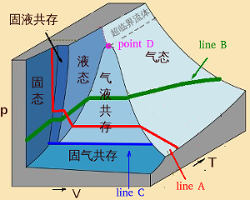
\includegraphics[width = 1.5in]{PVTdiagram.png}
\emini
}
\eitem
\ech
\end{frame}

\begin{frame}
\chtitle{典型的等压线和等温线}
\bch
\bmini{0.6}
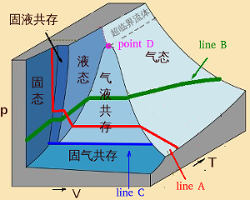
\includegraphics[width = 2.6in]{PVTdiagram.png}
\emini
\bmini{0.36}
{\small

\bitem
\item{典型的等压(加热)线:

 固态升温$\rightarrow$恒温熔化$\rightarrow$液态升温$\rightarrow$恒温汽化$\rightarrow$气态升温}

\item{典型的等温(压缩)线:

气态升压$\rightarrow$恒压液化$\rightarrow$液态升压$\rightarrow$恒压凝固$\rightarrow$固态升压

}
\eitem
}
\emini
\ech
\end{frame}


\begin{frame}
\chtitle{临界点}
\bch
\bitem
\item{\small 当我们逐步增加等温线的温度,气液共存线逐渐变短,直到缩为一个{\bf 临界点}。临界点的温度称为{\bf 临界温度$T_K$}。在温度为$T_K$的等温线上,液态和气态之间连续转化(没有体积跃变),且临界点为一个拐点,数学上即}
\eitem
\bmini{0.55}
\includegraphics[width = 2.2in]{PVTdiagram_TK.png}
\emini
\bmini{0.4}
{\small
$$\left(\frac{d p}{d V}\right)_{T=T_K} = \left(\frac{d^2 p}{d V^2}\right)_{T=T_K} = 0$$ 
\bitem
\item{$T>T_K$的等温线都是气态{\scriptsize(教材把超临界流体归类为气体,实际它也有部分液体性质)},所以在$T_K$以上不能通过等温压缩得到液态。}
\eitem
}
\emini
\ech
\end{frame}

\begin{frame}
\chtitle{三相共存线和三相点}
\bch
\bitem
\item{\small 当我们逐步减小等温线的温度,固液共存段和气液共存段的差别逐步减小,直到两者合并为一条线,即三相共存线。}
\eitem
\bmini{0.6}
\includegraphics[width = 2.6in]{PVTdiagram_T3.png}
\emini
\bmini{0.36}
{\small
\bitem
\item{当物质沿着三相共存线变化时,固液气三态并存,体积(以及三态物质的比例)发生变化,压强和温度都不变。}
\item{三相共存线对应的温度称为{\bf 三相点$\Tthree$}。按定义,水的三相点为$273.16\SIK$。}
\eitem
}
\emini
\ech
\end{frame}

\begin{frame}
\chtitle{$p$-$T$三相图}
\bch
\bmini{0.63}
\includegraphics[width = 2.6in]{PTdiagram.png}
\emini
\bmini{0.32}
{\small
把$p$-$V$-$T$曲面投影到$p$-$T$平面上,得到$p$-$T$三相图(也叫气液固三相图),可以很清楚地看出三相点不依赖于压强和体积。

从蒸发曲线上还可以直接读出{\bf 饱和蒸气压}(即气液共存时的压强)随温度的变化。}
\emini
\ech
\end{frame}

\begin{frame}
\chtitle{思考题}
\bch
\addfig{1}{think3.jpg}

早上经常看到的露珠是怎么形成的?
\ech
\end{frame}



\end{document}
